\subsection{Ledger}

In our payment design, we follow the Bitcoin paradigm in which all users maintain full and exclusive control of their monetary wealth through use of public key cryptography~\cite{nakamoto2008bitcoin}.
However, unlike Bitcoin, it is unnecessary for moneTor to rely on an inefficient decentralized consensus mechanism.
Since Tor already relies on a centralized set of authorities, we simply introduce a new ledger authority role to maintain the global payment state on a public tamper-evident database~\cite{crosby2009efficient}.
To maximize availability, this ledger may also be distributed across several authorities using, for example, the architecture proposed by RSCoin~\cite{danezis2015centrally}.
In principle, the ledger architecture is an orthogonal engineering problem.
We leave this challenge to the implementor and instead focus on the more critical design of off-ledger payment channels.

\subsection{Payment Protocols Overview}
\label{sec:payment_overview}

In this section, we specify formal protocols that comprise the moneTor payment infrastructure.
As first discussed Section~\ref{sec:background}, our chosen model is an implementation of the tripartite anonymous payment channel paradigm.
Compared to purely centralized schemes, payment channels are a critical method for scaling, allowing for a theoretically unbounded number of off-ledger transactions between any two parties.
However, in a na\"{i}ve two-party implementation, the total channel management complexity is on the order of $O(n \times m)$ where $n$ is the number of Tor clients and $m$ is the number of relays.
Our solution is to introduce the Intermediary Relay, a Tor node whose only role is to provide \emph{atomic} payment channel services between clients and relays.
By acting as trustless payment hubs maintaining persistent channels to many users, their services reduce the channel complexity to $O(n+m)$.
Notably, we can adjust the target number of intermediaries to balance the performance of the payment infrastructure and the size of the anonymity set for connected premium users.

\medskip \noindent\textbf{Bolt.} The basis of our scheme is an extension of Bolt's anonymous micropayment channel protocol, which is itself a privacy-focused adaption of the ``Lightning Network''~\cite{poon2016bitcoin}.
Due to its importance as a starting point for our work, we first provide a brief outline of the prerequisite micropayment channel procedures defined in Bolt.
All protocols are either two or three party interactions between a subset of the following roles: $C$ (client), $R$ (relay), $E$ (end-user: either a client or relay), $I$ (intermediary), and $L$ (ledger).
For our use case, the reader can assume that all communications are anonymously routed through Tor circuits~\cite{green2017bolt}.

\begin{itemize}
\item \textbf{KeyGen}: Generates a cryptographic keypair
\item \textbf{Init-E}: $E$ initializes half of a micropayment channel by
  escrowing funds on $L$
\item \textbf{Init-I}: $I$ initializes half of a micropayment channel by
  escrowing funds on $L$
\item \textbf{Establish}: $E$ and $I$ interact to establish a new micropayment
  channel from their respective halves
\item \textbf{Pay}: $C$ interacts with $I$ and $R$ to send a single micropayment to $R$
\item \textbf{Refund}: $E$ closes a channel on $L$ and makes a claim on
  the escrowed funds.
\item \textbf{Refute}: $I$ closes a channel on $L$ and makes a claim on
  the escrowed funds.
\item \textbf{Resolve}: $L$ determines the final balance of funds awarded to
  each party.
\end{itemize}

While anonymous micropayment channels present a tremendous advance for many applications, the relatively heavy cryptography (37-100 ms) and communication (7 messages) is a prohibitive expense, especially if we want to do it for every message transmission\footnote{In addition to concerns regarding global network overhead, it is also desirable to keep the barrier of entry low for smaller relay operators.}.
To overcome this barrier, we present a new payment layer design enabling far more efficient \emph{nanopayments} that will satisfy our constraints.

\medskip \noindent\textbf{moneTor.} The moneTor construction makes use of the existing anonymous micropayment structure to build \emph{locally transparent nanopayments}.
In this model, clients and relays extend single micropayment operations into \emph{nanopayment channels} through an intermediary (Figure~\ref{fig:parties}).
These highly lightweight channels allow the client to send $n$ unidirectional nanopayments to the relay through the established Tor circuit.
Each payment represents a fixed value $\delta$, established at the start of the channel.
By \emph{locally transparent}, we mean that each nanopayment in the same channel is trivially linked to each other.
However, the nanopayment channels themselves are unlinkable to other nanopayment channels and micropayment operations.
It is by design that this channel anonymity guarantee fits with Tor's existing circuit framework and security model, which similarly stipulates that messages within circuits are linkable internally but not externally to other circuits~\footnote{In contrast, as discussed in Section~\ref{sec:related_work}, some prior works implemented payments schemes which were needlessly unlinkable from the relay's viewpoint.}.
In essence, the overarching motivation of our work is to relax the costly anonymity guarantees provided by Bolt toward the design of a new set of protocols specifically adapted for Tor.
Finally, note that the establishments and closures of nanopayment channels do not require the clients or relay to interact with the ledger, resulting in a far more scalable design than any system which depends on resource-intensive centralized entities.

\begin{figure}[h] \centering
  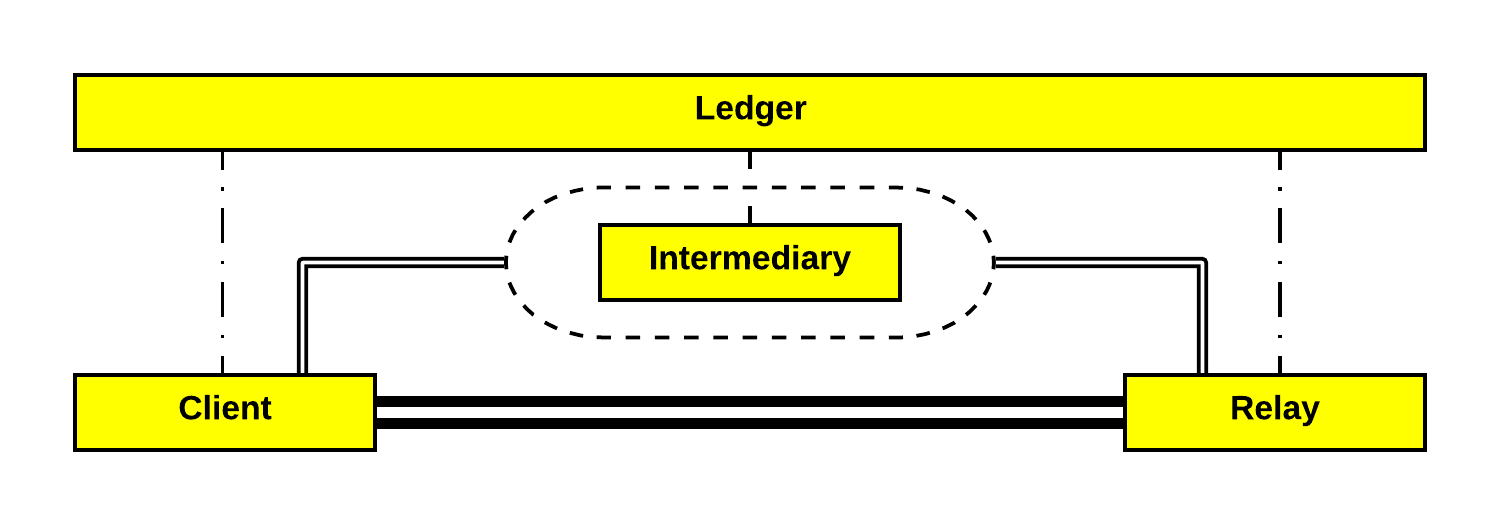
\includegraphics[trim={0.5cm, 0.5cm, 0.5cm, 0.5cm}, clip,
    scale=0.6]{images/party_diagram.png}
  \caption[Payment Roles]{Payment Roles --- Dashed lines represent periodic transactions (rare), thin double lines indicate micropayment channels (used at the beginning and end of circuit lifetime), and thick double lines indicate a nanopayment channel (handling nanopayments during the lifetime of the circuit).
    The dashed outline around the intermediary represents a notion of payment anonymity for the end-users.
    Connections to the ledger and to the intermediary are protected by an internal Tor circuit.}
  \label{fig:parties}
\end{figure}

We now briefly describe our new set of protocols.
Any two parties $C$ and $R$ can construct a nanopayment channel once both have completed Bolt's $Establish$ with a common intermediary $I$.
We define the following set of protocols needed to manage nanopayments:

\begin{itemize}
\item \textbf{Nano-Setup:} $C$ and $I$ interact to prepare an incomplete half of a nanopayment channel on top of their existing micropayment channel.
\item \textbf{Nano-Establish:} $C$ sends her nanopayment channel information to $R$, who interacts with $I$ to complete the second half of the nanopayment channel on top of their own existing micropayment channel.
\item \textbf{Nano-Pay:} $C$ sends a single nanopayment to $R$.
This is repeatable for up to $n$ operations.
\item \textbf{Nano-Close-R:} $R$ closes his nanopayment channel with $I$.
\item \textbf{Nano-Close-C:} $C$ closes her nanopayment channel with $I$.
This step must happen after \emph{Nano-Close-R}.
\end{itemize}

We also specify the following modified channel conflict resolution procedures to ensure secure closure properties for the nanopayment scheme.
Note that a
malicious party can force a closure (i.e., abort), but will not be able to steal anything thanks to the dispute resolution on the ledger.
It is important to note that the following algorithms run only in case of misbehaviour.

\begin{itemize}
\item \textbf{Nano-Refund:} $E$ closes the channel on $L$.
\item \textbf{Nano-Refute:} $I$ closes the channel on $L$.
\item \textbf{Nano-Resolve:} $L$ makes a final determination on both outstanding micropayment
  and nanopayment balances.
\end{itemize}

The core of our nanopayment scheme is inspired by the classic \emph{Payword} two-party micropayment scheme in which payments are encoded by successively revealed preimages in a precomputed hash chain~\cite{rivest1996payword}.

The challenge in this construction is to securely integrate the hash chain concept into an existing three-party anonymous micropayment channel setup such that all parties maintain secure cryptographic ownership of their funds at all steps.
At the same time, we must ensure the scheme does not leak deanonymizing information outside of the nanopayment channel context, a nontrivial task that requires significant restructuring of the Bolt protocol to fit our constraints.
Our final solution is a concrete scheme which incurs an overhead penalty of approximately two micropayment operations per nanopayment channel, one at the beginning and one at the end of the channel life cycle.

\subsection{Nanopayment Protocol Details}

\label{sec:nanopaymentdetails} In this section, we provide a summarized intuition for the basic steps in the payment protocol.
A more formal treatment of the steps are provided in Appendix~\ref{sec:algorithms} with algorithmic details.
Security considerations are detailed next in Section~\ref{subsec:paysecurity} and formally described in Appendix~\ref{sec:proof}.

\medskip \noindent\textbf{Nano-Setup} At the start of this protocol, $C$ has access to a micropayment wallet $w$ obtained from Bolt's \textbf{Establish} that enables her to operate her micropayment channel with the Intermediary $I$ as well as a refund token $rt$ that entitles her to claim her current funds on the ledger $L$ should $I$ misbehave or go offline.
To construct a nanopayment channel, $C$ first generates an array of values $hc$ of length $n$ where $hc_i = H(hc_{i+1})$ and $hc_n$ is a random number.
The root of the hash chain $hc_0$ is used to create a globally unique nanopayment token $nT$ that encodes the public parameters of the channel including the length $n$ and the per-payment value $\delta$.
$C$ sends $I$ a commitment to a fresh nanopayment channel parametrized by $nT$ along with a zero-knowledge proof of the following statements:

\begin{enumerate}
\item The nanopayment wallet $nw$ is well-formed from $w$.
\item $C$ has ownership of a micropayment channel containing at least $n \times \delta$ funds.
\end{enumerate}

$I$ verifies these messages and supplies $C$ with a new signed refund token $nrt$ that entitles $C$ to cash out the full balance of the micropayment channel using \textbf{Nano-Refund} if needed.
$C$, now protected against misbehavior by $I$, agrees to send a revocation token $\sigma_w$, which revokes her right to use $w$ to create other nanopayment channels from this micropayment wallet or to use $rt$ to cash out the micropayment channel before the \textbf{Nano-Close} is run.
$I$ is now protected against double spending by $C$ and can safely inform $C$ that the nanopayment channel has been set up successfully.

\medskip \noindent\textbf{Nano-Establish:} At this point, $C$ sends $R$ the same $nT$ token used to setup the channel with $I$.
$R$ uses the token to initiate her end of the nanopayment channel with $I$ by executing essentially the same procedure that $C$ used in \emph{Nano-Setup}.
The nanopayment channel is now fully established and ready to be used.
A key observation is that both ends of the channel ($C$-$I$ and $R$-$I$) are rooted at the same hash chain root $hc_0$.

\medskip \noindent\textbf{Nano-Pay:} To make the $i^{th}$ payment, $C$ simply sends the next hash preimage $hc_i$ to $R$.
Knowledge of this preimage $hc_i$ is sufficient for $R$ to prove possession of a nanopayment.
At any given time, $R$ can broadcast the tuple ($nrt$, $hc_i$) to $L$ to prove ownership of the correct balance of funds.
Notice that this action simultaneously reveals $hc_i$ to $I$, who can then claim an equivalent value of funds from $C$.
As a result, the scheme satisfies a correct-by-construction property of \emph{atomicity} whereby both legs of the protocol are finalized at the same time.

\medskip \noindent\textbf{Nano-Close:} After some number of payments $k < n$ has transpired and $C$ wants to close the Tor circuit, both $C$ and $R$ will generally prefer to close their nanopayment channels through $I$.
In this process, the $R$-$I$ leg must be closed before the $C$-$I$ leg.
This is due to the unidirectional nature of nanopayment channels.
Since payments are flowing from $C$ to $R$, $I$ must first determine its debt to $R$ in order to know how much it can claim from $C$.

$R$ first sends to $I$ a commitment to a new micropayment wallet $w'$ and a zero-knowledge proof of the following statements:

\begin{enumerate}
\item $w'$ is well-formed from $w$ ($w$ was either created by Bolt's establish phase or by a previous moneTor Nano-Close).
\item The balance of $w'$ is equal to the sum of the balance from the previous wallet $w$ and $\delta \times k$.
\end{enumerate}

Once verified, $I$ issues a refund token $rt'$ on the new funds.
$R$ agrees to invalidate the nanopayment channel by issuing a revocation token $\sigma_{nw}$ to $I$.
$I$ and $R$ proceed to create a blind signature on $w'$ thus validating the wallet for future use.

Once $I$ has closed his nanopayment channel leg with $R$, $I$ and $C$ are free to complete the exact same close protocol.
All parties now revert to the original state preceding \emph{Nano-Setup} save for a securely updated balance.

\medskip \noindent\textbf{Nano-Refund, Nano-Refute, Nano-Resolve:} Honest parties will not typically close active nanopayment channels on the ledger, opting instead to run Bolt micropayment closure procedures when they wish to cash out.
However, in the event of malicious behavior or premature abortion, \emph{Nano-Refund} and \emph{Nano-Refute} enable $E$ and $I$ to withdraw funds on the ledger with the latest payment information at any time.
After a set amount of time allowing for the counterparty to reciprocate, the ledger runs \emph{Nano-Resolve} to make a final publicly verifiable determination on the final balance.
Correct execution of these procedures allow all honest parties to retain their funds in some cases and obtain the full balance of the malicious party's escrowed funds in others.

\subsection{Payment Security and Anonymity} \label{subsec:paysecurity} Our security model must account for both privacy and payment security.
The privacy threat model derives from the local active adversary paradigm ubiquitously found in Tor research~\cite{dingledine2004tor}.
Like all cells in Tor, Nanopayment messages are locally linkable by relays participating in the circuit.
However, since each circuit is only ever associated with one anonymous nanopayment channel at any given time, relays and intermediaries cannot link two nanopayment channels with the same user.
Furthermore, Tor circuits protect all communication in the tripartite nanopayment protocol.
Hence, relationship between client to intermediary, client to ledger, relay to intermediary, and relay to ledger are themselves anonymized.
We provide formal definitions and proofs for the following theorem in Appendix~\ref{sec:proof}.

\begin{theorem}

  The nanopayment channel scheme offers anonymity (\ref{def:anon1}, \ref{def:anon2}) and secure balance (\ref{def:balance}) under the assumptions that the commitment scheme is secure, the zero-knowledge system is simulation extractable and zero-knowledge, and the hash function used to create the hashchain and verify the preimage during Nano-Pay is modeled as a random oracle.

\end{theorem}

This theorem fully covers the security and anonymity characteristics of the protocol leading up to the closing of a micropayment channel.
However, two points must be made with consideration to potential deanonymization after the conclusion of the protocol.
First, the price revealed to the ledger at micropayment close enables a subtle passive attack by $I$ which our security model does not capture.
By examining the final number of payments made on each channel in conjunction with the globally fixed nanopayment cost, $I$ may potentially link all of $C$'s nanopayment channels.\footnote{This attack is best illustrated with a trivial example.
Suppose that $I$ facilitates a number of nanopayment channels with the following number of payments, each of which is known to represent one unit of money: $[58, 839, 356, 881, 23, 89, 561]$.
Now $C$ closes her micropayment channel and terminates with exactly $58 + 356 = 414$ units of money.
Once the micropayment channel is closed, $I$ must necessary gain knowledge of the final balance of funds and can easily link the first and third nanopayment channels as belonging to the same $C$.}
To mitigate this vulnerability, we stipulate that $C$ must make at least one micropayment, which has a monetary value hidden from $I$, before closing a micropayment channel.
We expect that this micropayment should contain a random value not greater than the channel escrow maximum value as stated in the Tor consensus and may be made to another account owned by $C$.

Secondly, in the event of a dispute resolution on the ledger, the two parties on either end of the micropayment channel ($C$-$I$ or $I$-$R$), must disclose their on-ledger identities.
However, given an adequately privacy-preserving choice of an on-ledger transaction protocol such as Zerocash, even this result would be meaningless for $R$~\cite{sasson2014zerocash}.
Thanks to the built-in ledger privacy, $R$ can only link the ledger interaction to its circuit, but not to the client's real-world identity.

Having accounted for all privacy considerations both during and after the protocol, we informally state the following anonymity guarantees relative to unmodified Tor:

\begin{enumerate}
\item Additional parties needed to operate the moneTor system (i.e., ledgers and intermediaries) cannot extract any more information about a given client than any middle relay.
\item Excluding side channels, circuits do not leak any more information than the single bit needed to differentiate premium and nonpremium users.
\end{enumerate}

Our threat model for payment security is similar to those found in prior works in blockchain micropayment channels~\cite{poon2016bitcoin}.
In such models, the user is protected from malicious intermediaries by the ability to prove misbehavior to a global ledger.
Our protocols also guarantee that the client would not risk more money than initially agreed-upon (Balance property, see Section~\ref{def:balance}).

\medskip \noindent\textbf{Side-channels on Micropayment events.}
The moneTor protocol prescribes unlinkable micropayment events by protocol design.
However, a na\"{\i}ve implementation of this scheme may be susceptible to side-channel vulnerabilities, most notably, timing attacks.
For instance, a channel-creation policy that immediately mints a new nanopayment channel after the closing of the previous channel would allow $I$ to trivially link all channels belong to $C$.
To mitigate this particular risk, we require a random delay $t_r$ uniform $\in [0, r]$.
Since our scheme specifies the availability of preemptive channels, such a delay should not perversely impact user experience.
User privacy with respect to side channels and other statistical techniques depends on the number of users concurrently building channels to the same intermediary.
If we require an anonymity set of size $N$, then the maximum number of Intermediaries allowed in the network is $\frac{\mathbb{E}[W]}{N}$ where $W$ is a discrete random variable holding the number of payment events between any $t_i$, the time at \textbf{Nano-Close} and $t_{i+1}$, the time of the next \textbf{Nano-Setup} or \textbf{Nano-Establish}.
This number of events should be counted within a sliding time window of size $r$.
Consequently, the number of active Intermediaries should be a parameter of the system that the Tor project determines based on the activity of premium users.
Furthermore, clients should maintain channels with an number of different intermediaries to further mitigate any other unexpected side-channel leaks.

\subsection{Economic considerations}
\label{sec:economic_considerations}

Given the delicate nature of this research area, a key motivation in the technical design of our scheme is to explicitly accommodate some of the more consequential economic considerations.
For instance, in case of deployment, the Tor project would have to decide how to assign value to the moneTor tokens, a choice which entails fundamental trade-offs between control, liability, and social perception.
We enumerate three broad categories and briefly comment on the technical implementations as follows:

\begin{enumerate}

\item The Tor Project reserves control of monetary supply for the purpose of enforcing a publicly declared policy, for instance, to peg the value of tokens against one or more fiat currencies it that it holds in reserve.
This option would require the Tor Project to reserve a privileged signing key for minting new moneTor tokens (e.g.,
when a user makes fiat deposit).
\item The moneTor tokens are instantiated as a standard cryptocurrency whose value fluctuates as a function of market pressures and the chosen distribution schedule.
As an any cryptocurrency, a node that rejects the distribution mechanism (e.g.,
mining in Bitcoin) would be violating the protocol.
\item The moneTor tokens act as a secure wrapper for an external cryptocurrency such as Bitcoin, Ethereum, or a future state-backed currency.
This option is made possible by ongoing work in the field of ledger interoperability protocols~\cite{back2014enabling,poon2017plasma}.

\end{enumerate}

In all three cases, note that the mechanism required implement the police takes place entirely on the ledger.
Consequently, the off-ledger moneTor payment layer, which is the main contribution of this work, is compatible with any of these three options. 

Whereas the Tor Project has several acceptable options for monetary policy, there should not be such freedom in the pricing mechanism for premium bandwidth since any price differentiation between circuits would inevitably leak information.
This leakage becomes more severe with higher granularity payment options.
We therefore impose the constraint that all users should pay a single uniform price for premium bandwidth at any time $t$.

It is of course central to make sure that moneTor serves the goal of advancing of human rights and freedom of the Tor Project, which may be quite different from those that would result from a purely profit-seeking environment.
To this end, moneTor includes an explicit taxation mechanism, which we describe technically in Section~\ref{sec:tax_integration}.
Under this scheme, any time a payment takes place within the moneTor layer, a tunable fraction of the revenue is diverted into a special account controlled by the Tor Project.
This is analogous to a secure and automatic sales tax on premium traffic payments.
The Tor Project can use this fund to shape the topology of the network towards some notion of desirable diversity and performance via a transparent policy.
The exact content of such policy is an active subject of research that is orthogonal to our paper.\footnote{E.g., Waterfilling~\cite{waterfilling-pets2017} argues for security by maximum diversity in endpoints of user paths, and TAPS~\cite{taps-ndss2017} argues for security by trust policies.}
The tax rate also dictates incentives for nodes seeking to game the system, perhaps by inserting dummy traffic to collect tokens or faking bandwidth measurements.
We further elaborate on such questions and trade-offs in Section~\ref{sec:discussion}.

\subsection{Tax Integration}
\label{sec:tax_integration}

The zero-knowledge setup allows an elegant way to anonymously handle the tax collection policy.
Thus far, we have treated the nanopayment value $\delta$ as symmetric for both the client and relay leg.
In practice, it requires only a trivial modification to specify separate values of $\delta_C$ and $\delta_R$ such that the following equality is satisfied.

\begin{equation}
  \delta_C - \delta_R = \mathit{tax} + \mathit{fee}
  \label{eq:payment}
\end{equation}

\medskip \noindent Here, $\mathit{tax}$ is the portion of every payment that is redirected to the Tor tax authority while $\mathit{fee}$ represents compensation for $I$'s services.
$I$ gradually accumulates these overhead charges in his balance over the course of running many nanopayment channels.
When it is time for $I$ to cash out the full micropayment channel, $L$ simply divides the funds between the $I$ and the tax authority.
Note that this does \emph{not} mean that $L$ can arbitrarily control money as this process is well-defined in setup of the network protocol.

\subsection{Integration in Tor circuits}

Up to this point, we have described payments that occur between a single client and a single relay.
In practice, it is typical for each client to maintain a handful of concurrently active circuits,\footnote{For instance, the popular Tor Browser user application typically does not share circuits with streams targeting a different destination address unless those streams come from the same SOCKS connection.}
each of which requires three streams of payments to the guard, middle, and exit relays.
These channels must be actively managed to optimize computational overhead as well as money flow.
Furthermore, connections between the client and the guard relay are transparent and persistent across the timescale of several months.
We optimize toward this setup by enabling transparent and direct payment channels between the client and guard, considerably reducing the time to establish or close the channel.
In contrast, middle or exit relays channels require the flexibility of our full tripartite scheme. 

%%% Local Variables:
%%% mode: latex
%%% TeX-master: "../popets_monetor"
%%% End:
